\documentclass[a4paper,12pt]{article}
\usepackage{graphicx, float, enumerate, parskip}
\usepackage{amsmath, amssymb, amsthm}
\theoremstyle{definition}
\newtheorem{definition}{Definisi}[section]
\newtheorem{theorem}{Teorema}[section]
\newtheorem{example}{Contoh}[section]
\usepackage{listings, fancyvrb,  spverbatim, xcolor}
\lstset{% setup listings
    language=R,% set programming language
    frame=tb,
    basicstyle=\ttfamily\small,% basic font style
    keywordstyle=\color{blue},% keyword style
    commentstyle=\color{gray},% comment style
    breaklines=true,% automatic line breaking
    fancyvrb=true,% verbatim code is typset by listings
}
\usepackage[
    backend=biber,
    style=bwl-FU,
    sorting=nyt,
    maxbibnames=99,
    natbib=true,
]
{biblatex}
\addbibresource{DPustaka.bib}


%% ---------------------------
\begin{document}
    \title{Visualisasi Data Multivariat}
 \author{Kelompok 2: \\
    Yusnia Halimatussa'diyah 4112321007\\
    Fitria Adiba 4112321030\\}
\date{\today}
\begin{titlepage}
    \maketitle
\end{titlepage}

\section{Pendahuluan}
Topik visualisasi data multivariat berkaitan dengan materi yang lebih umum yang disebut \textit{exploratory data analysis} (EDA) atau analisis data eksplorasi dan grafik statistik. Istilah "\textit{exploratory}" berbeda dengan "\textit{confirmatory}", yang bisa menggambarkan pengujian hipotesis. Penting untuk melakukan pekerjaan eksplorasi sebelum pengujian hipotesis, dalam rangka mempelajari pertanyaan yang sesuai untuk diajukan serta metode yang paling tepat untuk menjawabnya. 

Pada bab ini beberapa fungsi grafik digunakan. Selain paket grafis R yang dimuat saat R dimulai, paket lain yang dibahas dalam bab ini adalah paket grafik \texttt{ggplot2} \cite{Wickham2016}, paket grafik \texttt{lattice trellis} \cite{Sarkar2008}, dan \texttt{MASS} [293]. Lihat juga antarmuka \texttt{rggobi} [174] ke Paket \texttt{GGobi} dan \texttt{rgl} [2] untuk visualisasi interaktif tiga dimensi (3D). Pada Tabel 5.1 dijelaskan fungsi grafik 2D dan beberapa metode visualisasi 3D.

Bab 1 memberikan ringkasan singkat tentang opsi warna, simbol plot, dan jenis garis.

\section{Tampilan Panel}
Tampilan panel adalah array ringkasan grafik dua-dimensi dari pasangan variabel pada data multivariat. Sebagai contoh, matriks scatterplot menampilkan scatterplot untuk semua pasangan variabel dalam suatu array. 

\begin{example}[Matriks Scatterplot]
    Empat variabel dibandingkan dalam data iris untuk spesies virginica, dalam matriks scatterplot.
    \begin{verbatim}
        data(iris)
        #virginica data in first 4 columns of the last 50 obs.
        pairs(iris[101:150, 1:4])
    \end{verbatim}
    Dalam plot yang dihasilkan oleh perintah \texttt{pairs} di atas, variabel nama akan muncul di sepanjang diagonal. Fungsi \texttt{pairs} mengambil opsional argumen \texttt{diag.panel}, yang merupakan fungsi yang menentukan apa yang ditampilkan disepanjang diagonal. Misalnya, untuk mendapatkan grafik dengan perkiraan kepadatan kurva sepanjang diagonal, berikan nama fungsi untuk memplot kepadatannya. Fungsi berikut dinamakan fungsi densitas dari \texttt{panel.d}.
    \begin{verbatim}
        panel.d <- function(x, ...) {
            usr <- par("usr")
            on.exit(par(usr))
            par(usr = c(usr[1:2], 0, .5))
            lines(density(x))
        }
    \end{verbatim}
    Pada \textbf{panel.d}, parameter grafik \textbf{usr} menentukan koordinat pengguna dari wilayah plotting. Sebelum memplot, diterapkan fungsi skala untuk menstandarkan masing-masing sampel satu dimensi.
    \begin{verbatim}
        x <- scale(iris[101:150, 1:4])
        r <- range(x)
        pairs(x, diag.panel = panel.d, xlim = r, ylim = r)
    \end{verbatim}
    Plot berpasangan ditampilkan pada Figure 2.1. Dari plot kita dapat mengamati bahwa variabel panjang berkorelasi positif, dan variabel lebar tampak berkorelasi positif. Struktur lain dapat muncul dalam data yang tidak dimunculkan oleh distribusi marjinal bivariat. Paket \textit{lattice} \citep{Sarkar2008}[258] menyediakan fungsi untuk membuat tampilan panel. Di sini diilustrasikan fungsi matriks scatterplot splom dalam \textit{lattice} untuk membuat tampilan panel.
    \begin{verbatim}
        library(lattice)
        splom(iris[101:150, 1:4]) #plot 1
        
        #for all 3 at once, in color, plot 2
        splom(iris[,1:4], groups = iris$Species)
        
        #for all 3 at once, black and white, plot 3
        splom(~iris[1:4], groups = Species, data = iris,
            col = 1, pch = c(1, 2, 3), cex = c(.5,.5,.5))
    \end{verbatim}
    Plot terakhir (plot 3) ditampilkan pada Figure 2.2. Ditampilkan di sini dalam warna hitam dan putih, tetapi pada layar tampilan panel lebih mudah diinterpretasikan saat ditampilkan berwarna (plot 2).
\end{example}

    \begin{figure}[H]
    \centering
    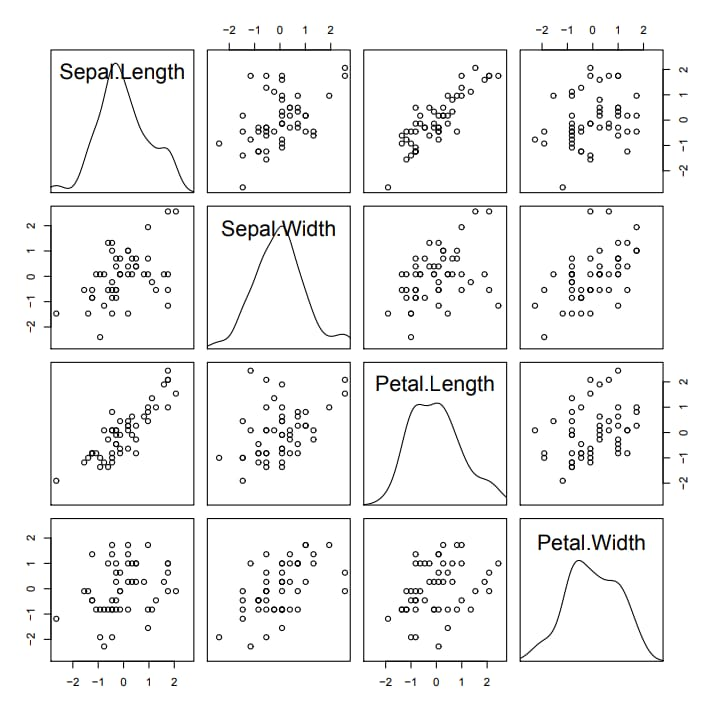
\includegraphics [width=8cm]{gb/K2G1}
    \caption{Scatterplot matrix (pairs) membandingkan empat pengukuran
    spesies iris virginica}
    \label{fig:my_label}
\end{figure}

\begin{figure}[H]
    \centering
    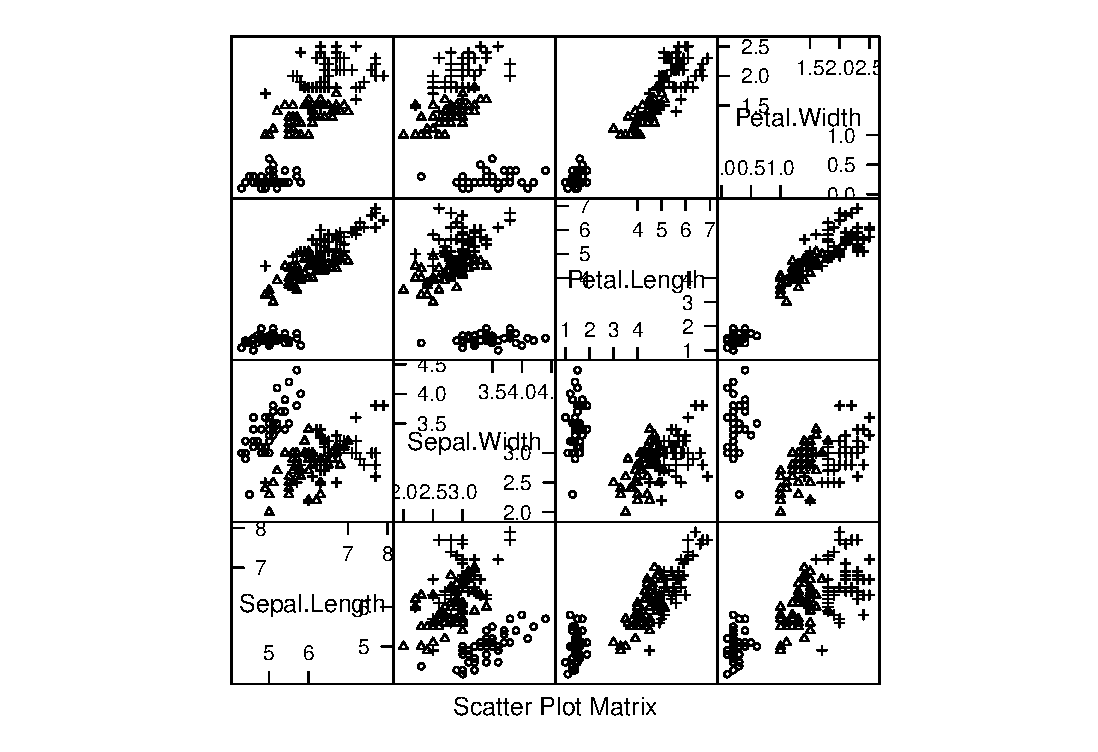
\includegraphics[width=16cm]{gb/K2G2-Scatterplot.pdf}
    \caption{Scatterplot matrix (pairs) membandingkan empat pengukuran
    spesies iris virginica, setosa (lingkaran), versicolor (segitiga), virginica (silang)}
    \label{fig:my_label}
\end{figure}

\section{Scatter Plot}
Jika dataset memiliki lebih dari empat atau lima variabel kuantitatif, maka susunan scatter plot seperti plot yang dihasilkan oleh \texttt{pairs} atau \texttt{splom} dalam \textit{lattice} tidak membantu untuk memvisualisasikan asosiasi berpasangan. Matriks korelasi selalu dapat dihitung, tetapi sebagian besar korelasi sulit untuk ditafsirkan. Ringkasan grafis dari korelasi berpasangan bisa sangat berguna dalam kasus ini.

Paket \texttt{corrplot} berisi fungsi \texttt{corrplot} untuk visualisasi dari matriks korelasi, bersama dengan fungsi pendukung yang memungkinkan untuk menyesuaikan urutan yang berbeda dari matriks. Fungsi \texttt{corrplot} memiliki banyak opsi, termasuk warna, bentuk, dan lain sebagainya yang dikontrol melalui beberapa argumen opsional.
\begin{example}[Data decathlon]
    Data decathlon disediakan dalam package \textit{FactoMineR} [178]
    Decathlon adalah kompetisi yang mencakup sepuluh cabang lintasan dan lapangan. Data Decathlon mencakup kinerja dari 41 atlet pada Pertandingan Olimpiade 2004 atau Decastar 2004, dengan peringkat dan poin yang dicetak. Misalkan kita tertarik pada asosiasi antara penampilan atlet di sepuluh nomor. Kami menghitung matriks korelasi untuk sepuluh variabel acara dan kemudian gunakan corrplot untuk menghasilkan plot untuk divisualisasikan matriks ini. Dari struktur fungsi str dapat dilihat bahwa sepuluh kejadian sesuai dengan sepuluh kolom pertama.

\begin{lstlisting}
library(FactoMineR) #decathlon data
library(corrplot)
data("decathlon")
str(decathlon)
corrMat <- cor(decathlon[, 1:10])
corrplot(corrMat, type="upper", tl.col="black", tl.srt=45)
}
\end{lstlisting}
\end{example}

\begin{figure}[H]
    \centering
    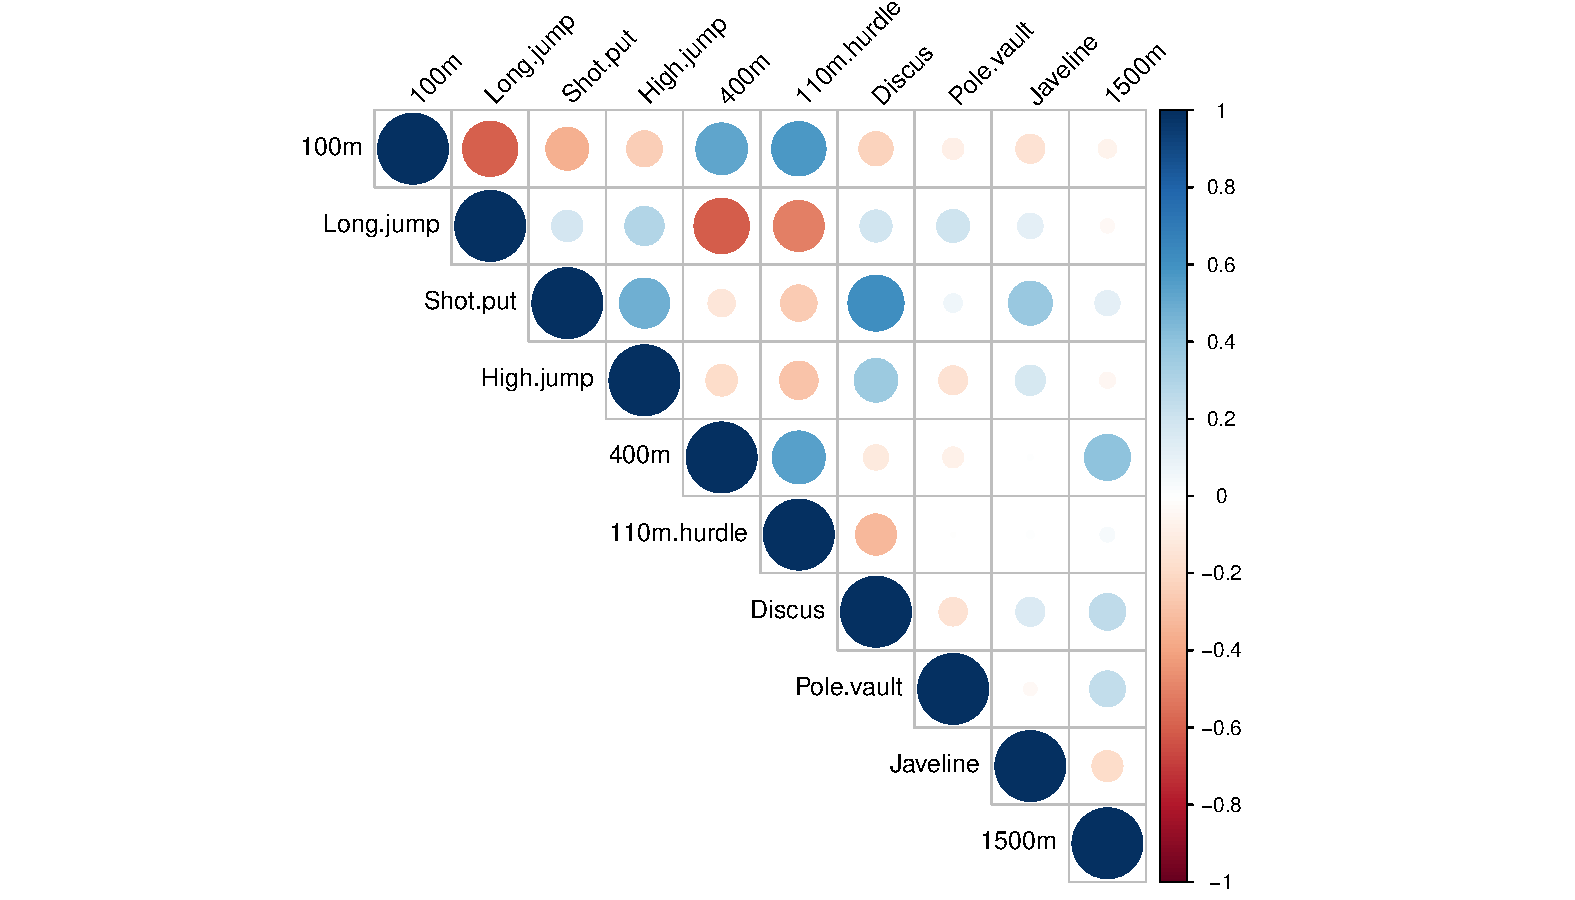
\includegraphics[width=16cm]{gb/K2G4-Scatterplot.pdf}
    \caption{Plot korelasi kinerja atlet dalam kejadian decathlon pada Contoh 3.1.}
    \label{fig:mesh1}
\end{figure}

Untuk menampilkan plot serupa dengan koefisien korelasi, kami menghapus
diagonal, ubah metode menjadi "square" dan gunakan addCoef.col = black
untuk koefisien.
\begin{lstlisting}
    corrplot(corrMat, type = "upper", method = "square",
addCoef.col = "black", diag=FALSE)

\end{lstlisting}
Dari plot yang dihasilkan pada Gambar 3.2 (lihat sisipan warna), kami memiliki kesamaan
visualisasi tetapi dengan ukuran simbol diganti dengan nilai
koefisien.

\begin{figure}[h]
    \centering
    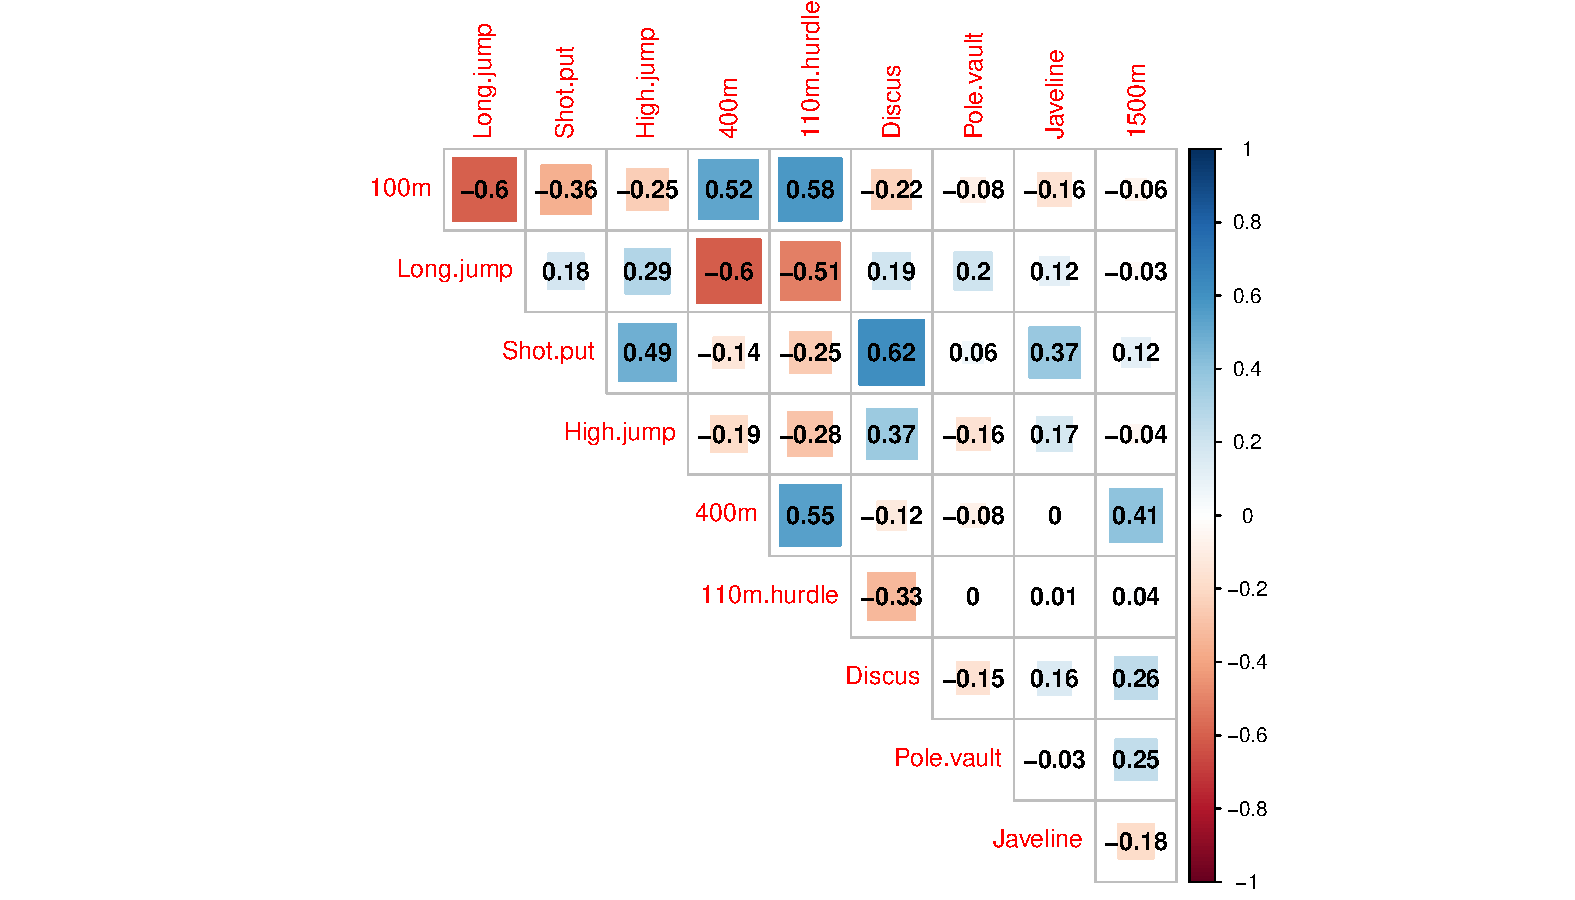
\includegraphics[width=16cm]{gb/K2G8-Scatterplot.pdf}
    \caption{Plot korelasi kinerja atlet dalam decathlon
peristiwa dengan koefisien korelasi, Contoh 3.1.}
    \label{fig:mesh1}
\end{figure}

\section{Plot Permukaan dan Scatter Plot 3D}
Beberapa packages menyediakan plot permukaan dan kontur plot. Fungsi \textit{perps}
(grafis) menggambar permukaan dari perspektif plot di atas bidang. coba jalankan contoh untuk \textit{perps}, untuk melihat banyak grafik yang menarik. 

\subsection{Plot Permukaan}
Untuk grafik tertentu kita perlu menyatukan kisi-kisi dari titik-titik yang berjarak teratur pada bidang. Perintah untuk ini adalah \texttt{expand.grid.} Jika tidak perlu kita simpan nilai \textit{x,y} dan hanya membutuhkan nilai fungsi $Z_{ij} = f(x_i, y_j)$,

\begin{example}[Plot Kepadatan Normal Bivariat]
\begin{equation}
    f(x,y)= \frac{1}{2\pi }e^{-{\tfrac{1}{2}}(x^{2}+y^{2})},  (x,y)\in \mathbb{R}^{2}
\end{equation}

Kode untuk permukaan plot densitas normal standar bivariat menggunakan fungsi \texttt{persp} dibawah ini. Sebagian besar parameter bersifat opsional; \texttt{x, y, z} diperlukan.
Untuk fungsi ini kita membutuhkan kisi lengkap dari nilai \textit{z}, tetapi hanya satu vektor
dari \textit{x} dan satu vektor dari nilai \textit{y}. Dalam contoh ini, $Z_{ij} = f(x_i, y_j)$ 
dihitung oleh fungsi luar.

\begin{lstlisting}
    #the standard BVN density
f <- function(x,y) {
z <- (1/(2*pi)) * exp(-.5 * (x^2 + y^2))
}
y <- x <- seq(-3, 3, length= 50)
z <- outer(x, y, f) #compute density for all (x,y)
persp(x, y, z) #the default plot
persp(x, y, z, theta = 45, phi = 30, expand = 0.6,
ltheta = 120, shade = 0.75, ticktype = "detailed",
xlab = "X", ylab = "Y", zlab = "f(x, y)")
\end{lstlisting}
\end{example}


\textbf{Menambahkan elemen ke plot perspektif}

Fungsi persp mengembalikan ‘viewing transformation' dalam matriks 4×4. Transformasi ini dapat digunakan untuk menambahkan elemen ke plot.

\begin{figure}[H]
    \centering
    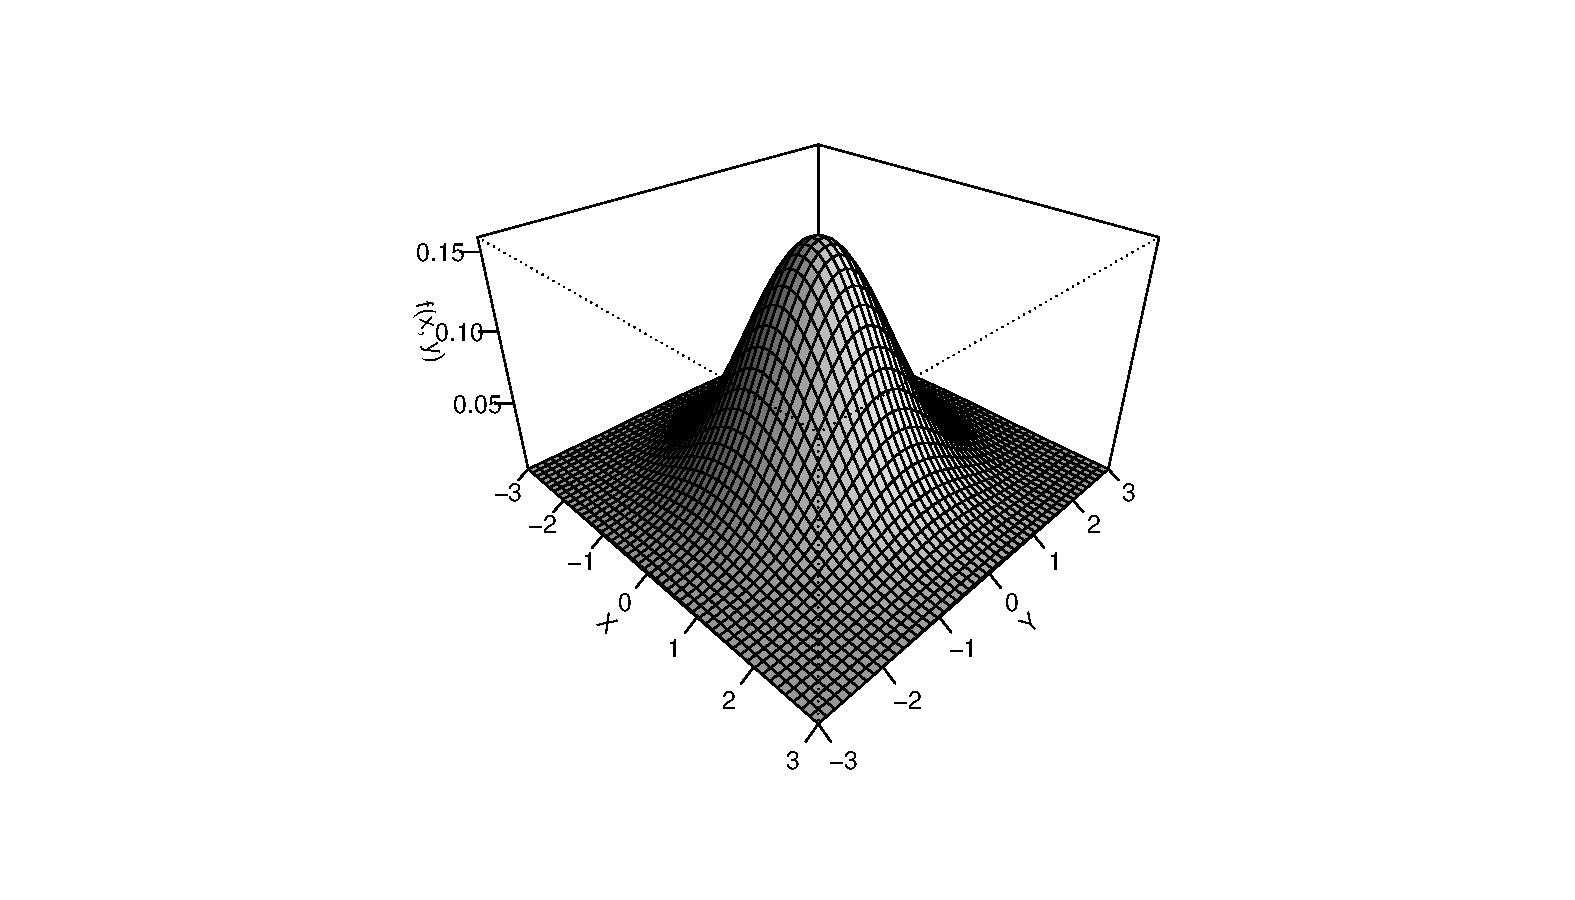
\includegraphics[width=16cm]{gb/K2G7-Scatterplot.pdf}
    \caption{Plot perspektif kepadatan normal bivariat standar}
    \label{fig:my_label}
\end{figure}

Example 5.4 (menambahkan elemen ke plot perspektif). Contoh ini menggunakan ‘viewing transformation’ dikembalikan oleh plot perspektif kepadatan normal bivariat standar untuk menambahkan titik, garis, dan teks ke plot.

\begin{lstlisting}
    #store viewing transformation in M 
persp(x, y, z, theta = 45, phi = 30, 
expand = .4, box = FALSE) -> M
\end{lstlisting}

Transformasi M ini diterapkan ke \texttt{x,y,z,t} untuk memproyeksikan titik ke layar
untuk ditampilkan dalam sistem koordinat yang sama yang digunakan untuk menggambar plot perspektif.
\begin{lstlisting}
    #add some points along a circle
a <- seq(-pi, pi, pi/16)
newpts <- cbind(cos(a), sin(a)) * 2
newpts <- cbind(newpts, 0, 1) #z=0, t=1
N <- newpts %*% M
points(N[,1]/N[,4], N[,2]/N[,4], col=2)
#add lines
x2 <- seq(-3, 3, .1)
y2 <- -x2^2 / 3
z2 <- dnorm(x2) * dnorm(y2)
N <- cbind(x2, y2, z2, 1) %*% M
lines(N[,1]/N[,4], N[,2]/N[,4], col=4)
#add text
x3 <- c(0, 3.1)
y3 <- c(0, -3.1)
z3 <- dnorm(x3) * dnorm(y3) * 1.1
N <- cbind(x3, y3, z3, 1) %*% M
text(N[1,1]/N[1,4], N[1,2]/N[1,4], "f(x,y)")
text(N[2,1]/N[2,4], N[2,2]/N[2,4], bquote(y==-x^2/3))
\end{lstlisting}

Plot dengan elemen tambahan ditunjukkan pada Gambar dibawah (Catatan: R menyediakan fungsi \texttt{trans3d} untuk menghitung koordinat di atas. Di sini kami telah menunjukkan perhitungan.)
\begin{figure}[H]
    \centering
    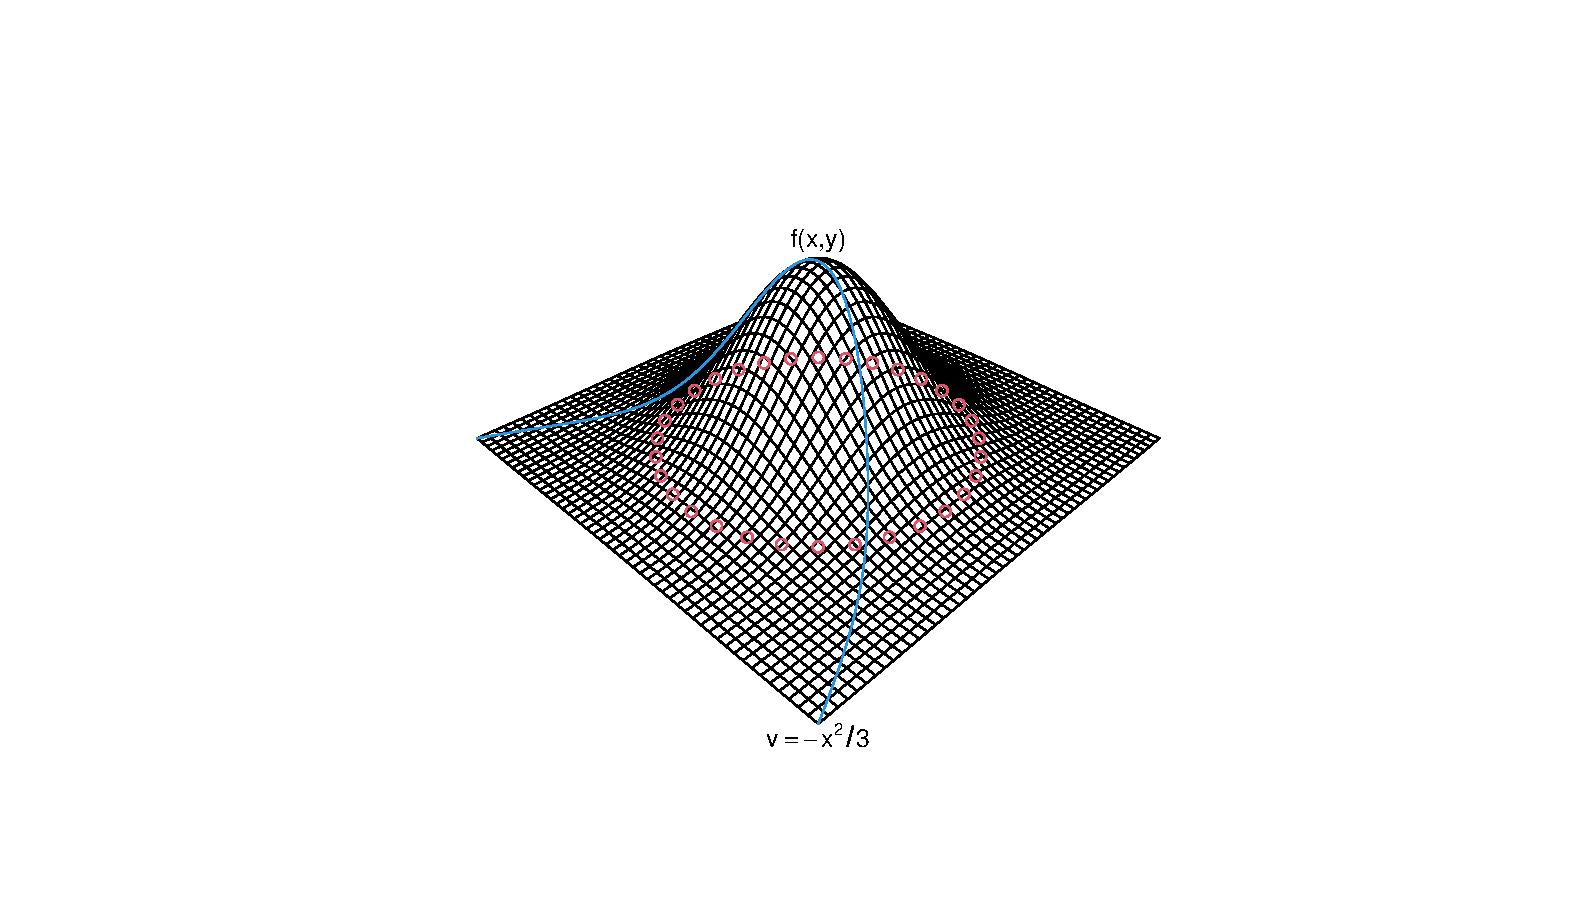
\includegraphics[width=16cm]{gb/K2G5-Scatterplot.pdf}
    \caption{Plot Perspektif dari kepadatan bivariat standar dengan elemen yang ditambahkan menggunakan transformasi yang di kembalikan oleh \texttt{persp}}
    \label{fig:my_label}
\end{figure}

\subsection{Scatter Plot Tiga Dimensi}

Fungsi \texttt{cloud} \texttt{lattice} \cite{Sarkar2008} menghasilkan scatter plot 3D. Mungkin penerapan jenis plot ini adalah untuk mengeksplorasi apakah ada kelompok atau cluster dalam data. Untuk menerapkan fungsi cloud, berikan rumus $z \sim  x* y$, di mana $z = f(x, y)$ adalah permukaan yang akan diplot. Bagian pertama berikut ini
adalah contoh aplikasi sederhana cloud dengan grup yang diidentifikasi berdasarkan warna. 
bagian kedua dari contoh mengilustrasikan beberapa opsi

\begin{example}[Contoh 5.1](scatter plot 3D). Contoh ini menggunakan fungsi cloud dipackage \texttt{lattice} untuk menampilkan scatter plot 3D dari data \texttt{iris}. Ada
tiga spesies iris dan masing-masing diukur pada empat variabel. Kode berikut menghasilkan scatter plot 3D panjang sepal, lebar sepal, dan panjang petal. 
\begin{lstlisting}
    library(lattice)
attach(iris)
#basic 3 color plot with arrows along axes
print(cloud(Petal.Length ~ Sepal.Length * Sepal.Width,
data=iris, groups=Species))
\end{lstlisting}

Data \texttt{iris} memiliki empat variabel, jadi ada empat himpunan bagian dari tiga variabel
untuk membuat grafik. Untuk melihat keempat plot di layar, gunakan opsi \texttt{more} dan \texttt{split}.
\texttt{split} argumen menentukan lokasi plot di dalam panel. 

\begin{lstlisting}
print(cloud(Sepal.Length ~ Petal.Length * Petal.Width,
data = iris, groups = Species, main = "1", pch=1:3,
scales = list(draw = FALSE), zlab = "SL",
screen = list(z = 30, x = -75, y = 0)),
split = c(1, 1, 2, 2), more = TRUE)
print(cloud(Sepal.Width ~ Petal.Length * Petal.Width,
data = iris, groups = Species, main = "2", pch=1:3,
scales = list(draw = FALSE), zlab = "SW",
screen = list(z = 30, x = -75, y = 0)),
split = c(2, 1, 2, 2), more = TRUE)
print(cloud(Petal.Length ~ Sepal.Length * Sepal.Width,
data = iris, groups = Species, main = "3", pch=1:3,
scales = list(draw = FALSE), zlab = "PL",
screen = list(z = 30, x = -55, y = 0)),
split = c(1, 2, 2, 2), more = TRUE)
print(cloud(Petal.Width ~ Sepal.Length * Sepal.Width,
data = iris, groups = Species, main = "4", pch=1:3,
scales = list(draw = FALSE), zlab = "PW",
screen = list(z = 30, x = -55, y = 0)),
split = c(2, 2, 2, 2))
detach(iris)
\end{lstlisting}
\end{example}

Keempat scatterplot 3D ditunjukkan pada Gambar 5.7. Plot menunjukkan itu tiga spesies \texttt{iris} dipisahkan menjadi kelompok atau kelompok dalam subruang tiga dimensi yang dibentang oleh tiga dari empat variabel. Ada beberapa struktur jelas dalam plot ini. Seseorang dapat menindaklanjuti dengan analisis kluster atau analisis komponen utama untuk menganalisis struktur yang tampak di dalam data.
menampilkan.

\begin{figure}[H]
    \centering
    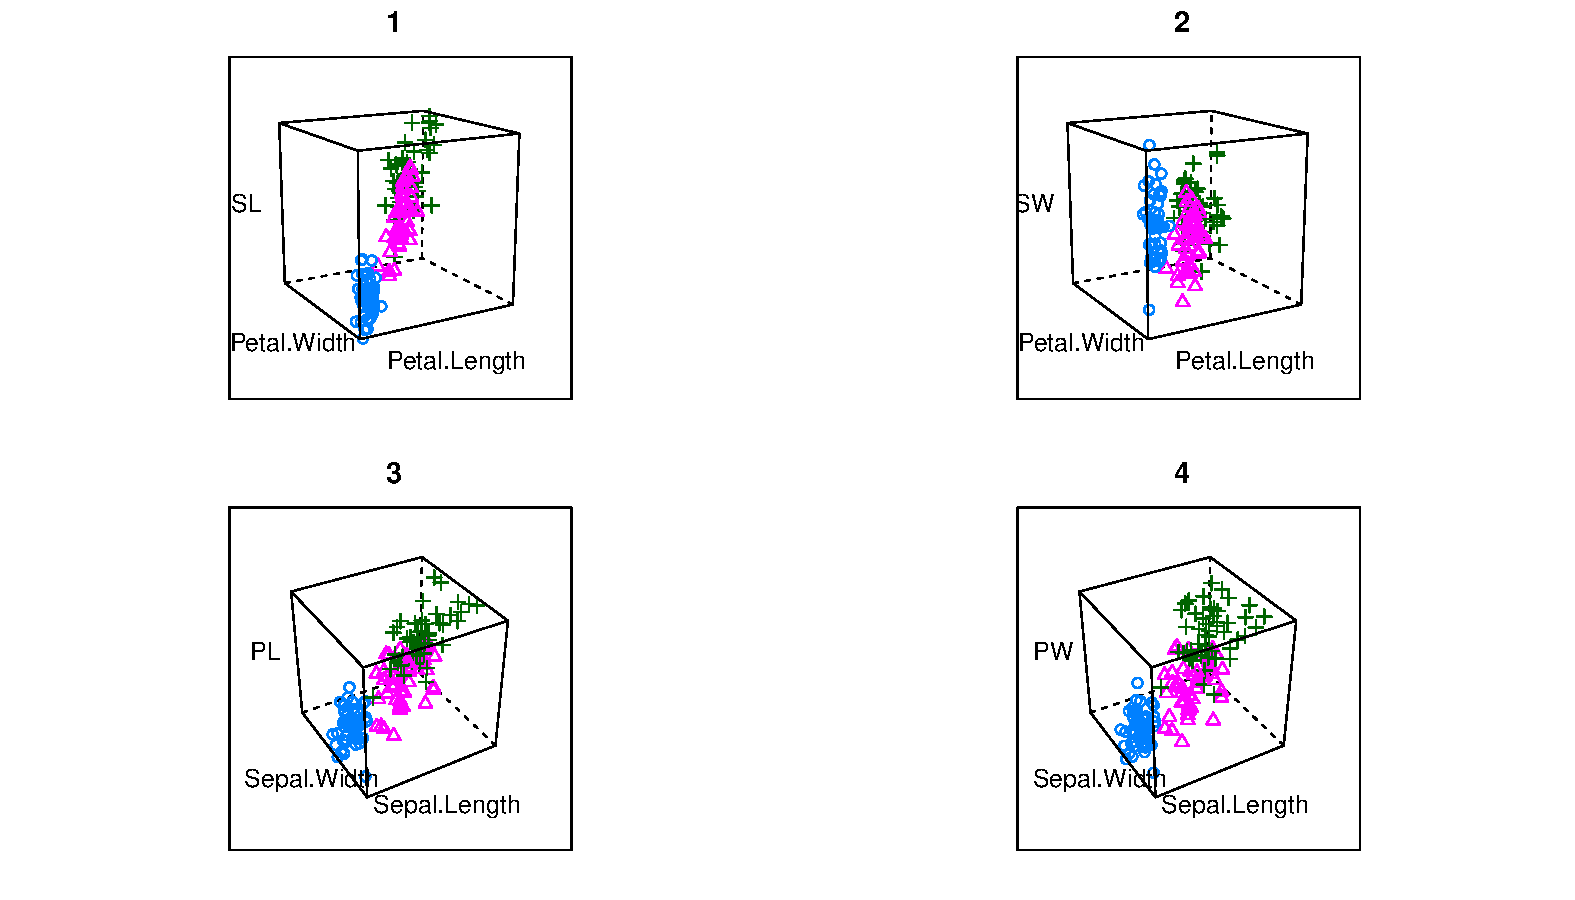
\includegraphics[width=16cm]{gb/K2G6-Scatterplot.pdf}
    \caption{Scatter Plot 3D dari data iris yang dihasilkan oleh \texttt{cloud} \texttt{(lattice)} dengan masing-masing spesies diwakili oleh karakter plot yang berbeda.}
    \label{fig:my_label}
\end{figure}



\section{Latihan}
\begin{enumerate}
\item Bangkitkan 300 pengamatan acak dari distribusi normal multivariat yang memiliki vektor mean $\mu = (0, 1, 2)$ dan matriks kovarians
\[
\Sigma = \begin{bmatrix}
1.0 & -0.5 & 0.5\\ 
-0.5 & 1.0 & -0.5\\ 
0.5 & -0.5 & 1.0
\end{bmatrix}
\]
Buatlah matriks scatterplot dan verifikasi bahwa lokasi dan korelasi untuk setiap plot sesuai dengan parameter distribusi bivariat yang dibangkitkan.

\item
Tambahkan kurva halus yang cocok untuk masing-masing Scatterplot pada Gambar 5.1 dari
Contoh 5.1. (?\texttt{panel.smooth})
\item

\item Buatlah plot kontur berisi campuran bivariat pada Latihan 5.3.
\item Buatlah plot permukaan campuran bivariat pada Latihan 5.3
\item Ulangi Latihan 5.3 untuk berbagai pilihan dari parameter yang berbeda
model campuran, dan bandingkanlah distribusi melalui plot kontur.
\item Buat plot koordinat paralel dari data \texttt{crabs} (MASS) [293] menggunakan
semua 200 pengamatan. Bandingkan plot sebelum dan sesudah menyesuaikan
pengukuran dengan ukuran \texttt{crabs}. Tafsirkan plot yang dihasilkan.





\end{enumerate}



\newpage
\printbibliography[heading=bibintoc,title={Daftar Pustaka}]
\end{document}